\section{Zahlenmengen}
\setcounter{page}{1}

\begin{figure}[h]
\centering
	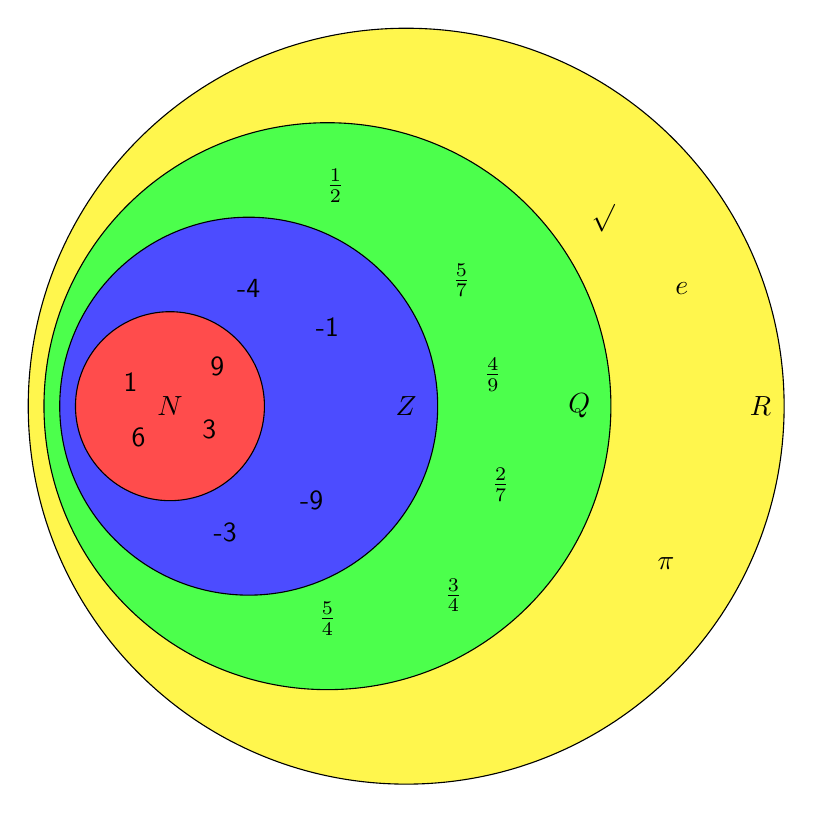
\begin{tikzpicture}[font=\sffamily]
  % Zentrale Punkte für die Positionierung der Beschriftungen
  \coordinate (N) at (-3,0);
  \coordinate (Z) at (0,0);
  \coordinate (Q) at (2.2,0);
  \coordinate (R) at (4.5,0);
  \coordinate (C) at (6.6,0);
  
  % Konzentrische Kreise
  \draw[fill=yellow!70] (0,0) circle (4.8cm); % R
  \draw[fill=green!70] (-1,0) circle (3.6cm); % Q
  \draw[fill=blue!70] (-2,0) circle (2.4cm);  % Z
  \draw[fill=red!70] (-3,0) circle (1.2cm);   % N
  

  % Beschriftungen
  \node at (N) {$\mathbb{N}$};
  \node at (Z) {$\mathbb{Z}$};
  \node at (Q) {$\mathbb{Q}$};
  \node at (R) {$\mathbb{R}$};
  
   % Zahlenbeispiele
  % Natürliche Zahlen N
  \node at (-3.5,0.3) {1};
  \node at (-2.5,-0.3) {3};
  \node at (-3.4,-0.4) {6};
  \node at (-2.4,0.5) {9};

  % Ganze Zahlen Z
  \node at (-1,1) {-1};
  \node at (-2,1.5) {-4};
  \node at (-1.2,-1.2) {-9};
\node at (-2.3,-1.6) {-3};
  
  % Rationale Zahlen Q
  \node at (-0.9,2.8) {$\frac{1}{2}$};
  \node at (0.6,-2.4) {$\frac{3}{4}$};
  \node at (-1,-2.7) {$\frac{5}{4}$};
  \node at (1.1,0.4) {$\frac{4}{9}$};
  \node at (1.2,-1) {$\frac{2}{7}$};
  \node at (0.7,1.6) {$\frac{5}{7}$};
  
  % Reelle Zahlen R
  \node at (2.5,2.4) {$\sqrt{}$};
  \node at (3.3,-2) {$\pi$};
  \node at (3.5,1.5) {$e$};
  
\end{tikzpicture}
\end{figure}
\begin{itemize}
	\item [$\mathbb{N}$] Die Zahlenmenge der natürlichen Zahlen beinhaltet alle positiven Zahlen, die kein Dezimalbruch sind
	\item [$\mathbb{Z}$] Die Zahlenmenge der ganzen Zahlen beinhaltet alle Zahlen der vorherigen Zahlenmenge inklusive negativer Zahlen
	\item [$\mathbb{Q}$] Die Zahlenmenge der rationaler Zahlen beinhaltet alle Zahlen der vorherigen Zahlenmenge inklusive Dezimalbrüche und Brüche
	\item [$\mathbb{R}$]  Die Zahlenmenge der reelen Zahlen beinhaltet alle Zahlen der vorherigen Zahlenmenge inklusive Zahlen wie $pi$, $e$ und 
\end{itemize}
\pagebreak
